\documentclass[thesis.tex]{subfiles}
\begin{document}

\chapter{Survival Processes in Pancreatic Cancer}
\label{ch:prognostic}

Outline ideas:
\begin{itemize}
  \item Overall thesis for this work: That specific molecular processes control survival following PC resection, and that these processes are not apparent from examining CPVs, but can be identified and detected using GEX data.
  \item Introduction
  \begin{itemize}
    \item General background on outcome with PC, with focus on post-op.  Make the note of the wide range of survival times.  Segue into reasons for this variability...
    \item Background on predictive CPVs in PC.  MSKCC.
    \item What is known about molecular risk factors so far?
    \begin{itemize}
      \item There are some very specific cases, eg HER2
      \item On more broad sigs, there are some (eg Collisson), but:
      \begin{itemize}
        \item Generated backwards, generally by unsupervised clustering
        \item Cluster-based sigs don't appropriately capture smooth varying states, eg stroma content.
      \end{itemize}
    \item Wrap-up.  Range of survival in PC is high, and is \emph{not} well-explained by known effects.  This is probably a consequence of the ad-hoc approach used to identify processes.  Thesis: that distinct molecular processes are determining survival in PC.  Set to find these using modern techniques.  Allude to future -- that these processes may point to new therapeutic directions and also are useful simply for staging (or maybe keep this point for the conclusion)
    \end{itemize}
  \end{itemize}
  
  \item Methods
  \begin{enumerate}
    \item Cohort recruitment and ethics (if this is the first survival chapter, else just reference the previous one)
    \item Sample prep and GEX wet lab
    \item Normalization, standardization, cohort subsetting, etc
    \item Filtering.  Unsupervised $\rightarrow$ Van-ISIS $\rightarrow$ AdaEN/SCAD/EN.  Select latter based on CV IBS, due to instability of AdaEN/SCAD.  What about TIE*?
    \item DR: Induce modules (APC) or metagenes (PCA).  Can investigate sparse PCA as intermediate method.
    \item Functional assignation.  Statnikov multiplicity problem.  GSVA or similar on MSigDB, also on sigs from above.  Correlate.
    \item Sanity checking.  Perform the above filtering and DR steps on permuted data.  Verify that the distribution of correlations with non-permuted signatures is as random as expected.
  \end{enumerate}
  
  \item Results
  \begin{enumerate}
    \item Cohort characteristics (if first surv chapter)
    \item Filtering metrics.  Unsup, ISIS, penalized.  Report CV IBS for penalized methods.
    \item DR.  Number of components / clusters with best CV IBS.
    \item Function.
  \end{enumerate}

  \item Conclusion
\end{itemize}

\section{Introduction}

\section{Methods}
\subsection{Cohort recruitment and ethics}
\mpfatal{CPVs current as of 4 Nov 2014}

\subsection{Sample collection, preparation, and gene expression microarrays}
\mpfatal{}
End with saved as \gls{IDAT} files.  241 of them (class 7 with CPVs only)

\subsection{Data preprocessing}
\paragraph{Microarray quality control and normalization}
\gls{IDAT} files were read into Bioconductor \texttt{lumi} structures using the \texttt{lumidat} package.  Seven arrays were excluded on the basis of poor signal, due to fewer than 30\% of probes on these arrays having detection P-values of less than 0.01.  The remaining 234 microarrays represented a range of tumour types, and were normalized as one batch using the \texttt{lumi} package.  Normalization proceeded serially as: RMA-like background subtraction (\texttt{lumiB} method \texttt{"bgAdjust.affy"}), VST (\texttt{lumiT} method \texttt{"vst"}), and quantile normalization (\texttt{lumiN} method \texttt{"quantile"}).

\paragraph{Unsupervised probe selection}
Probes were excluded if they met any of the following criteria: fewer than 10\% of samples with expression P-values of less than 0.01, a probe quality (from the \texttt{illuminaHumanv4PROBEQUALITY} field in Bioconductor package \texttt{illuminaHumanv4.db}) not equal to `perfect' or `good', missing gene annotation, or a standard deviation of normalized expression values across all samples of less than 0.03.  The choice of this latter threshold is expected to yield approximately a 5\% false probe rejection rate, based on an analysis of the variation between technical replicate samples.  In cases where multiple post-filter microarray probes mapped to the same gene, only the probe with the highest standard deviation, as evaluated across all samples that passed quality checks, was retained.  The effect of these combined filtering steps was to reduce the number of features under consideration from 47,273 probes to 13,000, one per gene.

\paragraph{Sample selection}  From the full set of 234 tumour samples that passed quality checks, eight were from four samples that had each been arrayed twice, and two were from patients with multiple conflicting \gls{CPV} data.  The two with conflicting \gls{CPV} data were excluded from further study, and the eight replicated samples were averaged, after \gls{MDS} indicated that each replicate pair had very similar expression.

\paragraph{Summary}
The above preprocessing steps yielded matched \gls{CPV} and resected tumour \gls{GEX} data for 13,000 genes across 228 patients.

\subsection{GSVA scoring}


\subsection{Outcome-associated gene selection}

Genes that were associated with either disease-specific survival or time to progression were identified by \gls{SIS} operating on the \gls{FAST} statistic \cite{Gorst-Rasmussen2013}, with a \gls{CPSS} wrapper to reduce the false positive rate \cite{Shah2013}.  Figure \ref{fig:surv_varsel} depicts the selection methodology, in which \gls{FAST}-\gls{SIS} selection was applied to three clinical intervals: time from diagnosis to recurrence, time from recurrence to disease-specific death, and time from diagnosis to disease-specific death.  Genes chosen by any one of the three \gls{FAST}-\gls{SIS} procedures were deemed selected by the wrapping procedure, the intuition underlying this inclusive criterion being that the biology affecting the progression of pre- and post-recurrence disease may be different.  Each \gls{FAST}-\gls{SIS} selector provided 325 outcome-associated genes, and 50 rounds of the wrapping \gls{CPSS} procedure were used, with parameter $\tau = 0.72$.  213 of 13,000 genes were deemed to be outcome-associated by this process, giving $\hat{\theta} = 0.048$ and therefore an expected bound on the number of false positive genes of 10 (equivalent to $FDR \leq 0.05$) \cite{Shah2013}. \mpfatal{Results?}

\begin{figure}
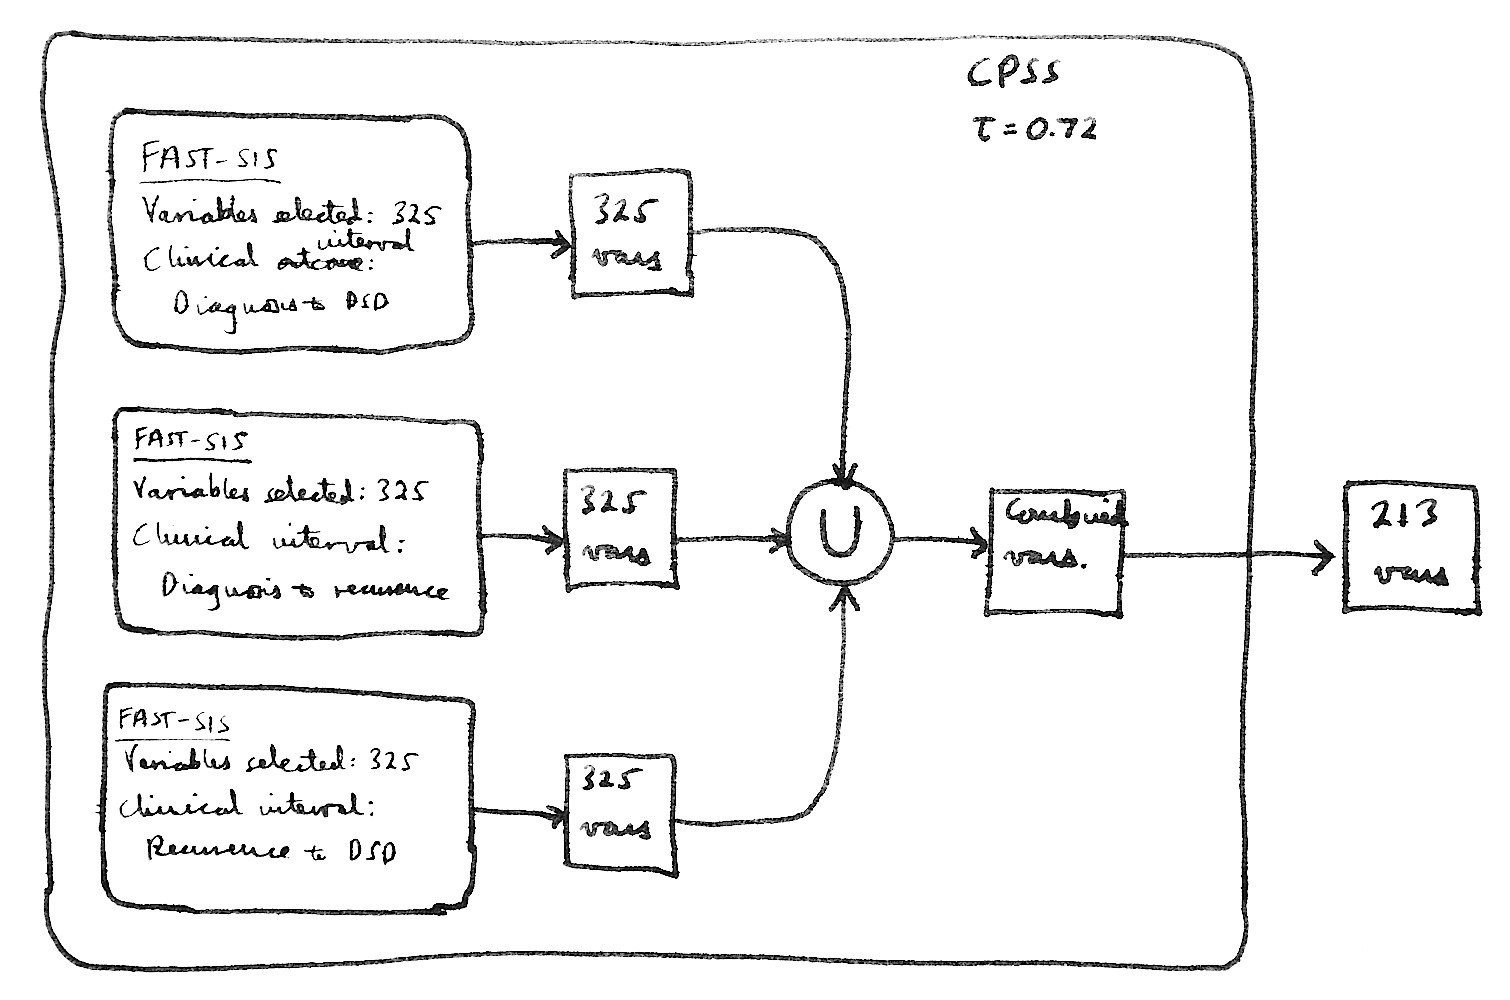
\includegraphics[width=100mm]{resources/surv_varsel.jpg}
\caption{Outcome-associated variable selection methodology.  325 genes were selected by each of three \acrshort{FAST}-\acrshort{SIS} blocks, each identifying genes associated with time from either diagnosis to death, diagnosis to recurrence, or recurrence to death.  A union was then made of genes selected by the three \acrshort{FAST}-\acrshort{SIS} blocks to yield a combined gene set.  This entire selection procedure was wrapped within 50 rounds of \acrshort{CPSS}, which yielded the final stability-selected set of 213 outcome-associated genes.}
\label{fig:surv_varsel}
\end{figure}

\subsection{Rank estimation and metagene factorization}
The gene x patient expression matrix of outcome-associated genes was decomposed into metagenes by the SNMF/L procedure of \cite{Kim2007}, implemented in a custom R package by the author.  Factorization rank was estimated following \cite{Frigyesi2008}: for test ranks ranging from 2 to 15, 10 SNMF/L decompositions were performed, each on a permuted version of the expression matrix.

\subsection{Metagene functional characterization}

\section{Results}
\subsection{}
\subsection{Linking metagenes to biology}

\section{Discussion}

\bibliographystyle{plain}
\bibliography{thesis}

\end{document}
